\documentclass{article}  % Define la clase del documento.

% Paquetes de idioma y codificación
\usepackage[utf8]{inputenc}
\usepackage[T1]{fontenc}
\usepackage[spanish]{babel}  % Ajusta el idioma del documento a español.

% Paquete de geometría para configurar márgenes y tamaño de papel
\usepackage[letterpaper, margin=3cm]{geometry}

% Paquetes de tipografía
\usepackage{mathptmx}    % Usa Times New Roman como fuente.
\usepackage{microtype}   % Mejora la justificación del texto.

% Paquetes para manejo de colores y gráficos
\usepackage{xcolor}      % Define y utiliza colores.
\usepackage{graphicx}    % Permite la inserción de imágenes.
\usepackage{tikz}        % Creación de gráficos vectoriales.

% Configuración de enlaces y referencias cruzadas
\usepackage{hyperref}
\hypersetup{
    colorlinks   = true,
    linkcolor    = darkblue,
    citecolor    = black,
    filecolor    = blue,
    urlcolor     = blue
}

% Paquetes para la mejora visual de tablas y figuras
\usepackage{booktabs}    % Para tablas de alta calidad.
\usepackage{float}       % Controla la posición de figuras y tablas.

% Paquete para la personalización de códigos fuente
\usepackage{listings}
\lstset{
    literate=
    {á}{{\'a}}1 {é}{{\'e}}1 {í}{{\'i}}1 {ó}{{\'o}}1 {ú}{{\'u}}1
    {Á}{{\'A}}1 {É}{{\'E}}1 {Í}{{\'I}}1 {Ó}{{\'O}}1 {Ú}{{\'U}}1
    {ñ}{{\~n}}1 {Ñ}{{\~N}}1 {ü}{{\"u}}1 {Ü}{{\"U}}1,
    backgroundcolor=\color{backcolour},
    commentstyle=\color{codegreen},
    keywordstyle=\color{codepurple},
    numberstyle=\tiny\color{codegray},
    stringstyle=\color{red},
    basicstyle=\ttfamily\small,
    breakatwhitespace=false,
    breaklines=true,
    captionpos=b,
    keepspaces=true,
    numbers=left,
    numbersep=5pt,
    showspaces=false,
    showstringspaces=false,
    showtabs=false,
    tabsize=2,
    language=TeX,
    morecomment=[l]\#,
    frame=single,
    rulecolor=\color{black}
}

% Definición de colores al estilo Visual Studio Code
\definecolor{darkblue}{rgb}{0.0, 0.0, 0.55}  % Enlaces
\definecolor{codegreen}{rgb}{0.25, 0.49, 0.48}  % Comentarios
\definecolor{codegray}{rgb}{0.5, 0.5, 0.5}  % Números y anotaciones
\definecolor{codepurple}{rgb}{0.58, 0, 0.82}  % Palabras clave
\definecolor{backcolour}{rgb}{0.95, 0.95, 0.92}  % Fondo de código

% Configuraciones de párrafo y matemáticas
\usepackage{amsmath}
\usepackage{parskip}    % Espaciado entre párrafos.
\usepackage{ragged2e}   % Justificación mejorada.

% Configuración de secciones y encabezados
\usepackage{titlesec}
\titleclass{\part}{top} % Make part like a class
\titleformat{\part}[display]
  {\normalfont\huge\bfseries\centering}{\thepart}{40pt}{\Huge}
\titlespacing*{\part}{178pt}{-60pt}{10pt}
\titleformat{\part}
  {\normalfont\huge\bfseries}{}{0pt}{}

% Asegúrate de usar esto para mantener el estilo en las páginas de las partes
\titleformat{\part}[display]
  {\normalfont\huge\bfseries}{}{0pt}{}
  [\thispagestyle{fancy}] % Aplica el estilo fancy a las páginas de las partes

% Configuración de encabezados y pies de página personalizados
\usepackage{fancyhdr}
\pagestyle{fancy}
\fancyhf{}
\fancyhead[L]{\raisebox{0.20cm}{\textbf{Métodos Computacionales en Obras Civiles}}}
\fancyhead[R]{\raisebox{0.1cm}{
\includegraphics[width=0.25\linewidth]{LOGO_UNIVERSIDAD.jpg}}}
\fancyhead[C]{\rule{\textwidth}{0.6pt}}
\fancyfoot[C]{\rule{\textwidth}{0.6pt}}
\fancyfoot[R]{\raisebox{-1.5\baselineskip}{\thepage}}
\renewcommand{\headrulewidth}{0pt}
\renewcommand{\footrulewidth}{0pt}

% Configuración avanzada de geometría
\geometry{
  top=3.5cm, % Aumenta el espacio en la parte superior para subir el encabezado
  bottom=2.5cm,
  headheight=2.5cm % Aumenta la altura del encabezado si es necesario
}

% Configuracion de bibliografia
\usepackage{natbib}
\bibliographystyle{unsrtnat}  % Puedes cambiarlo por `unsrtnat`, `abbrvnat`, etc.

\begin{document}
%----------------------------------------------------------------------------------------
% PORTADA
%----------------------------------------------------------------------------------------
\begin{titlepage}%Inicio de la carátula, solo modificar los datos necesarios
\newcommand{\HRule}{\rule{\linewidth}{0.5mm}} 
\center 
%----------------------------------------------------------------------------------------
%	ENCABEZADO
%----------------------------------------------------------------------------------------

\includegraphics[width=10cm]{LOGO_UNIVERSIDAD.jpg}\\ % Si esta plantilla se copio correctamente, va a llevar la imagen del logo de la facultad.OBS: Es necesario incluir el paquete: graphicx
\vspace{3cm}
%----------------------------------------------------------------------------------------
%	SECCION DEL TITULO
%----------------------------------------------------------------------------------------
\HRule \\[0.4cm]
{ \huge \bfseries Entrega 0, Proyecto 1}\\[0.4cm] % Titulo del documento
{ \huge \bfseries Metodos Computacionales en OOCC, IOC 4201}\\[0.4cm] % Titulo del documento
\HRule \\[1.5cm]
 \vspace{5cm}
%----------------------------------------------------------------------------------------
%	SECCION DEL AUTOR
%----------------------------------------------------------------------------------------
\begin{flushright}
    { \textbf{Profesor:}\\
    Patricio Moreno\\
    \vspace{0.2cm}
    \textbf{Ayudante:} \\
    Maximiliano Biasi\\
    \vspace{0.2cm}
    \textbf{Alumno:} \\
    Lukas Wolff Casanova\\
}
\end{flushright}
\vspace{1cm}
%----------------------------------------------------------------------------------------
%	SECCION DE LA FECHA
%----------------------------------------------------------------------------------------
{\large \textbf{\today}}\\[2cm] % El comando \today coloca la fecha del dia, y esto se actualiza con cada compilacion, en caso de querer tener una fecha estatica, reemplazar el \today por la fecha deseada
\end{titlepage}
%----------------------------------------------------------------------------------------
%  INDICE
%----------------------------------------------------------------------------------------
\newpage
\thispagestyle{empty} % Deshabilita el número de página en la página del índice
\tableofcontents
\thispagestyle{plain} % Deshabilita el encabezado en la página del índice
\thispagestyle{empty} % Deshabilita el número de página en la página del índice
\newpage

\newpage
\thispagestyle{empty}
\listoffigures 
\thispagestyle{plain} % Deshabilita el encabezado en la página del índice %
\thispagestyle{empty}
\newpage
%----------------------------------------------------------------------------------------
%ACÁ EMPIEZA EL INFORME
\setcounter{page}{1}
%----------------------------------------------------------------------------------------
\part{Entrega 0}
\begin{center}
  \href{https://github.com/LukasWolff2002/PROYECTO_1_MCOCo}{Ver repositorio en GitHub}.
\end{center}

\section{Introducción}

Una ataguía, también llamada cofre, es un recinto construido dentro o a través de un cuerpo de agua para permitir que el área cerrada sea bombeada \textbf{\citet{acerlum2023}}.
\\ \\
De esta manera, se determina que el análisis estructural y geomecánico de una ataguía es fundamental, no solo para determinar cuánto caudal es necesario extraer, sino también para garantizar la seguridad en la zona de trabajo, donde hay factores como la presión de poros o licuefacción del suelo que hay que tomar en consideración.
\\ \\
En base a lo anteriormente mencionado, se desarrolló un análisis para una ataguía en 3 casos distintos, determinando así cuál es el más idóneo a utilizar.

\section{Marco Teórico}

A continuación se presentarán las distintas ecuaciones utilizadas en el desarrollo del informe.

\subsection{Infiltración}

\begin{equation}
  I = k \cdot h_l \cdot \frac{N_i}{N_d} \cdot 24 \cdot 3600 [m^3/día]
\end{equation}

Donde $N_d$ es el número de redes de flujo y $N_i$ es el número de líneas equipotenciales.

\subsection{Presión de Poros}

\begin{equation}
  u = \frac{h_p \cdot \gamma_{agua}}{1000} [KPa]
\end{equation}

\begin{equation}
  h_p = \Delta H_i - Z_g
\end{equation}

\begin{equation}
  \Delta H_i = h_i - \frac{\Delta H \cdot n_i}{N_d}
\end{equation}

Y $Z_g$ corresponde a la altura del punto en la línea equipotencial, $h_i$ a la altura inicial, $\Delta H$ al gradiente hidráulico, $n_i$ al número de línea equipotencial y $N_d$ al número de redes de flujo.

\subsection{Máximo Gradiente Hidráulico}

Corresponde a la mínima distancia que debe recorrer el agua, es decir;

\begin{equation}
  G = \frac{\Delta h_{min}}{L}
\end{equation}

\subsection{Falla por Licuefacción}

Para conocer si falla por licuefacción, primero es necesario calcular $i_c$:

\begin{equation}
  i_c = \frac{\gamma_{suelo} - \gamma_{agua}}{\gamma_{agua}}
\end{equation}

Luego se determina si falla por licuefacción si $i_c < G$.

\subsection{Factor de Seguridad}

Finalmente, el factor de seguridad se calcula como:

\begin{equation}
  FS = \frac{G}{i_c}
\end{equation}

\section{Desarrollo}

Los códigos escritos y utilizados se encuentran en el siguiente enlace: \href{https://github.com/LukasWolff2002/PROYECTO_1_MCOC/tree/main/CODIGO}{Código Python}. Por efectos de simplicidad del informe, estos no serán explicados en detalle.

\subsection{Esquemas}

\begin{figure}[H]
  \centering
  \begin{minipage}{0.32\textwidth}
      \centering
      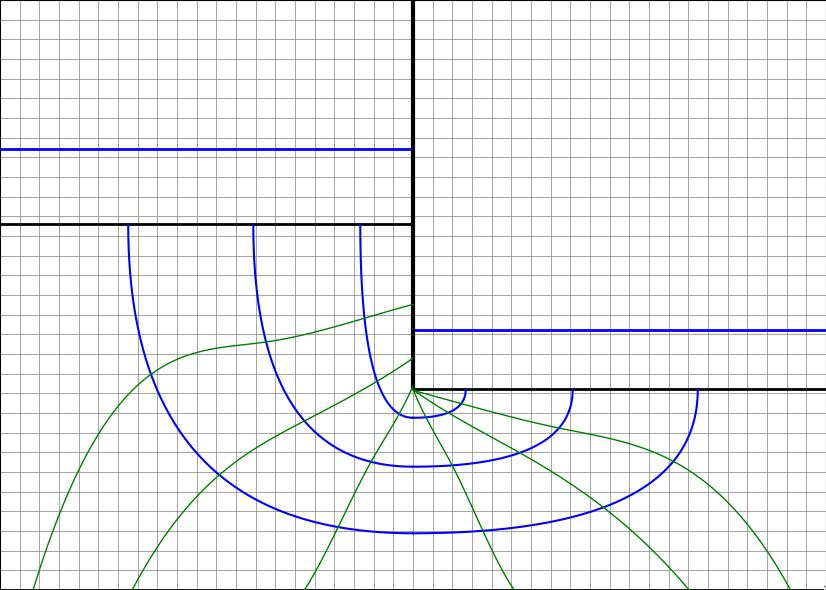
\includegraphics[width=\textwidth]{FOTOS/caso_1dibujo_base.jpg}
      \caption{Caso 1 Base}
  \end{minipage}
  \begin{minipage}{0.32\textwidth}
      \centering
      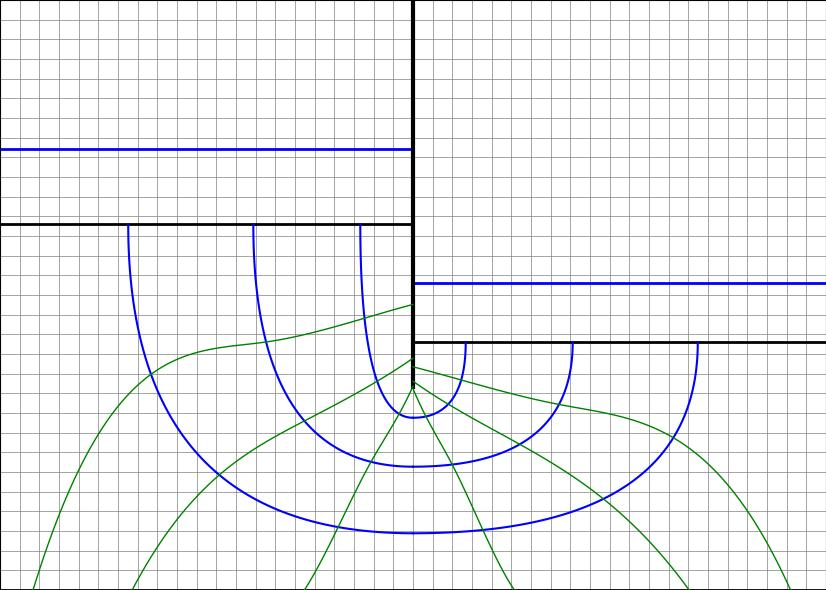
\includegraphics[width=\textwidth]{FOTOS/caso_2dibujo_base.jpg}
      \caption{Caso 2 Base}
  \end{minipage}
  \begin{minipage}{0.32\textwidth}
      \centering
      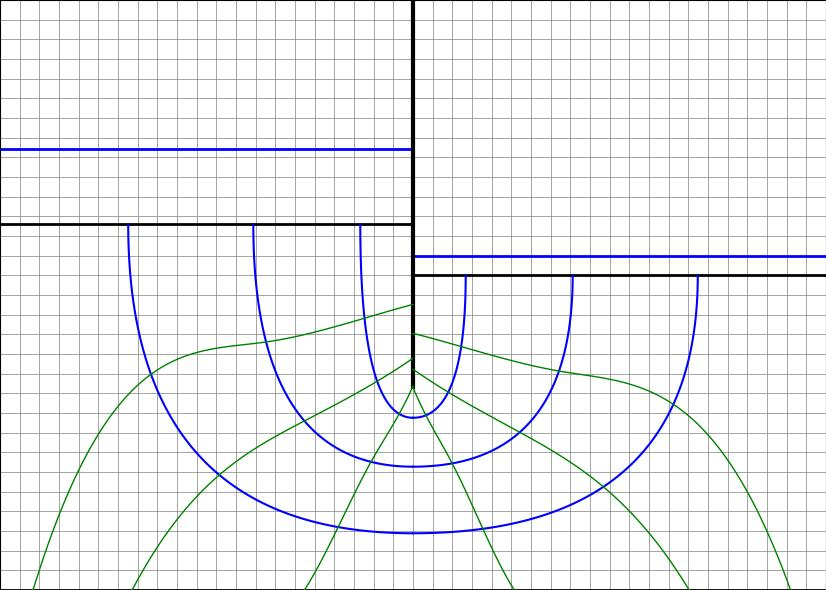
\includegraphics[width=\textwidth]{FOTOS/caso_3dibujo_base.jpg}
      \caption{Caso 3 Base}
  \end{minipage}
\end{figure}

Los dibujos en tamaño A4, como fue solicitado, y con un espaciado de 5mm (en escala correspondiente a 1 metro), se encuentran en el siguiente enlace: \href{https://github.com/LukasWolff2002/PROYECTO_1_MCOC/tree/main/DIBUJOS_A4}{Esquemas A4}.
\\ \\
\textbf{Nota:} Los dibujos fueron realizados en Python, utilizando distintas librerías para poder lograr la equipotencialidad. En base a las coordenadas obtenidas, se realizaron los distintos cálculos.

\subsection{Caudal de Infiltración}

Se calculó el caudal de infiltración como:

\begin{lstlisting}[language=Python]
  hl = (C1+B1) - (C2+B2)
  inf = k*hl*(num_canales/(num_equipotenciales))*24*3600 #m3/dia
\end{lstlisting}

Lo cual dio como resultado:

\begin{table}[H]
  \centering
  \begin{tabular}{|c|c|}
    \hline
    Caso & Caudal de Infiltración [$m^3/dia$] \\
    \hline
    1 & 20.567 \\ \hline
    2 & 15.202 \\ \hline
    3 & 12.072 \\
    \hline
  \end{tabular}
  \caption{Caudal de Infiltración}
  \label{fig:Q_inf}
\end{table}

\subsection{Presión de Poros}

Se define como la presión ejercida por una columna de agua desde la profundidad de la formación hasta el nivel freático \textbf{\cite{por2024}}.

\subsection{Presión Ataguía}

\subsubsection{Presiones Totales}

\begin{figure}[H]
  \centering
  \begin{minipage}{0.32\textwidth}
      \centering
      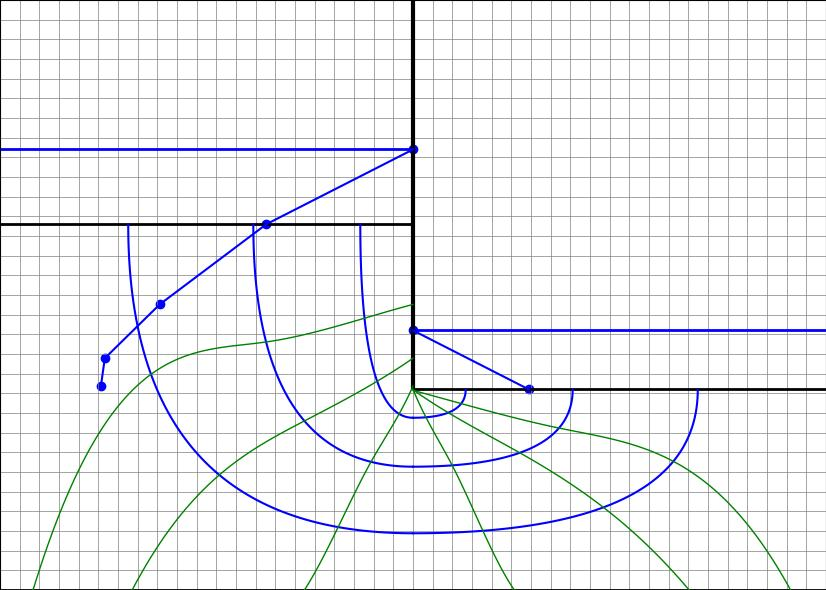
\includegraphics[width=\textwidth]{FOTOS/caso_1_presion_ataquia_total.jpg}
      \caption{Caso 1 Presiones Ataguía}
  \end{minipage}
  \begin{minipage}{0.32\textwidth}
      \centering
      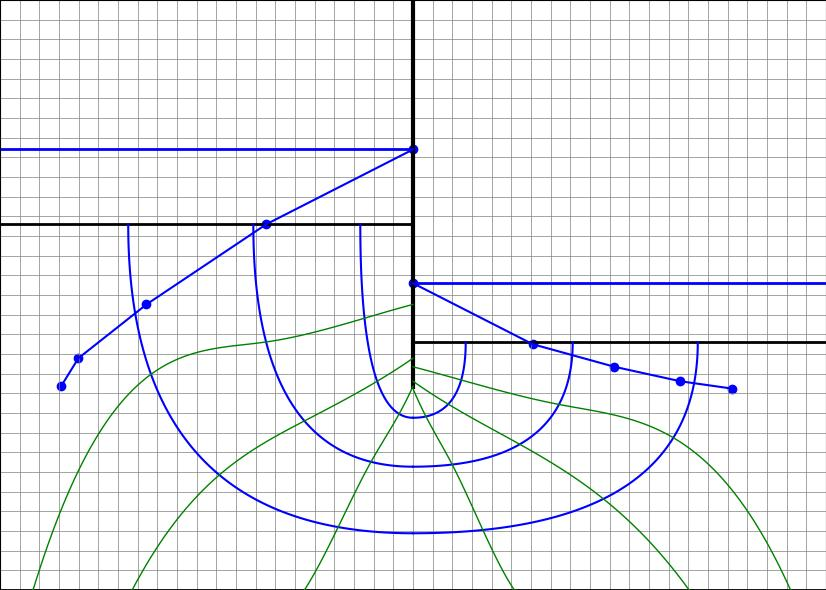
\includegraphics[width=\textwidth]{FOTOS/caso_2_presion_ataquia_total.jpg}
      \caption{Caso 2 Presiones Ataguía}
  \end{minipage}
  \begin{minipage}{0.32\textwidth}
      \centering
      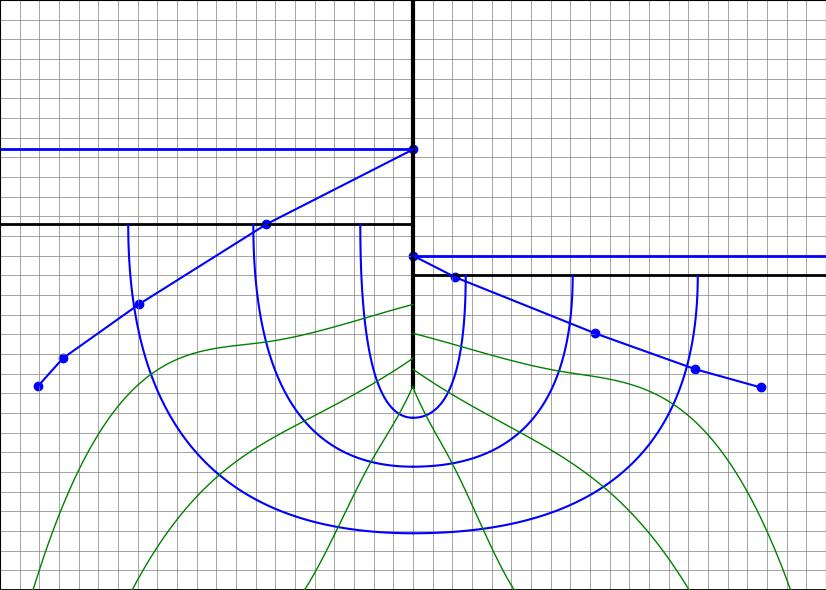
\includegraphics[width=\textwidth]{FOTOS/caso_3_presion_ataquia_total.jpg}
      \caption{Caso 3 Presiones Ataguía}
  \end{minipage}
\end{figure}

Donde las presiones en los distintos puntos solicitados son:

\begin{table}[H]
  \centering
  \begin{tabular}{|c|c|c|c|c|c|c|c|c|}
    \hline
    Caso & A & B & C & D & E & F & G & H \\
    \hline
    1 & 0 & 37.28 & 71.14 & 79.33 & 79.35 & 68.13 & 27.47 & 0 \\ \hline
    2 & 0 & 37.28 & 59.70 & 78.65 & 89.44 & 81.17 & 27.47 & 0 \\ \hline
    3 & 0 & 37.28 & 50.01 & 56.37 & 95.33 & 88.45 & 7.85 & 0 \\
    \hline
  \end{tabular}
  \caption{Presiones en Ataguía [KPa]}
\end{table}

Para calcular estas presiones, primero se calcularon las presiones en los distintos puntos conocidos de las líneas piezométricas:

\begin{lstlisting}[language=Python]
  #Primero calculo el delta H, el cual debe ser en metros
  Delta_H = (C1+B1) - (C2+B2)

  #Luego calculo Z, el cual es la altura para el gráfico obtenido
  #a partir de una lista de coordenadas, por lo tanto, 
  #convierto las coordenadas a metros.
  z = ((coor[clave][1]-altura_rel)*200)/1000

  #Calculo Zg
  Zg = z

  #Luego calculo ni, el número de línea equipotencial
  ni = int(clave.split('_')[1])

  #En base a esto, es posible obtener delta_hi
  Delta_Hi = (C1+B1)-((Delta_H*ni)/Nd)

  #Calculo hp
  hp = Delta_Hi-Zg

  #Y finalmente U en [KPa]
  u = (hp*gamma_agua)/1000
  
  #Este proceso es aplicado en todos los puntos conocidos
  
\end{lstlisting}

Posteriormente, aplico una regresión lineal a la curva obtenida y así calculo las presiones en los distintos puntos solicitados.

\begin{lstlisting}[language=Python]
  from scipy.interpolate import interp1d

  interpolacion = interp1d(x_known, y_known, kind='linear')
\end{lstlisting}

En base a todas las presiones de poros conocidas, fue posible aplicar un mapa de calor:

\subsubsection{Mapa de Presión}

\begin{figure}[H]
  \centering
  \begin{minipage}{0.32\textwidth}
      \centering
      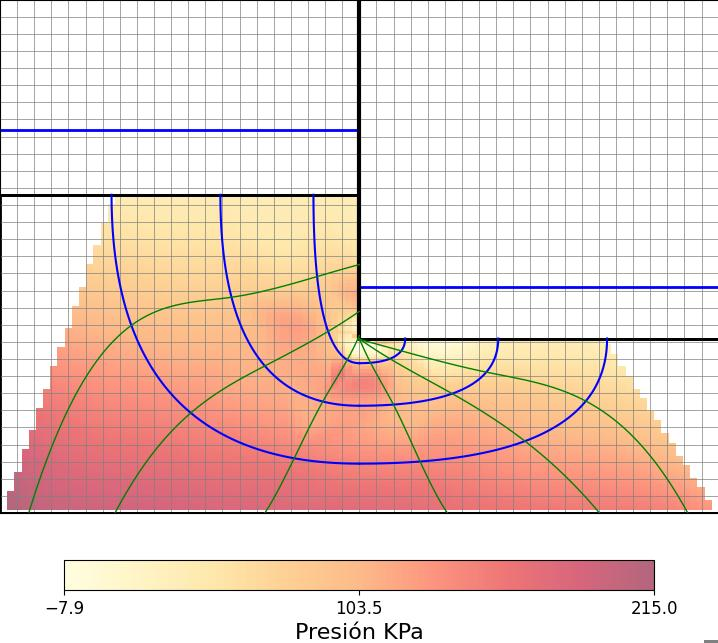
\includegraphics[width=\textwidth]{FOTOS/caso_1_mapa_calor.jpg}
      \caption{Caso 1 Presiones de Poros}
  \end{minipage}
  \begin{minipage}{0.32\textwidth}
      \centering
      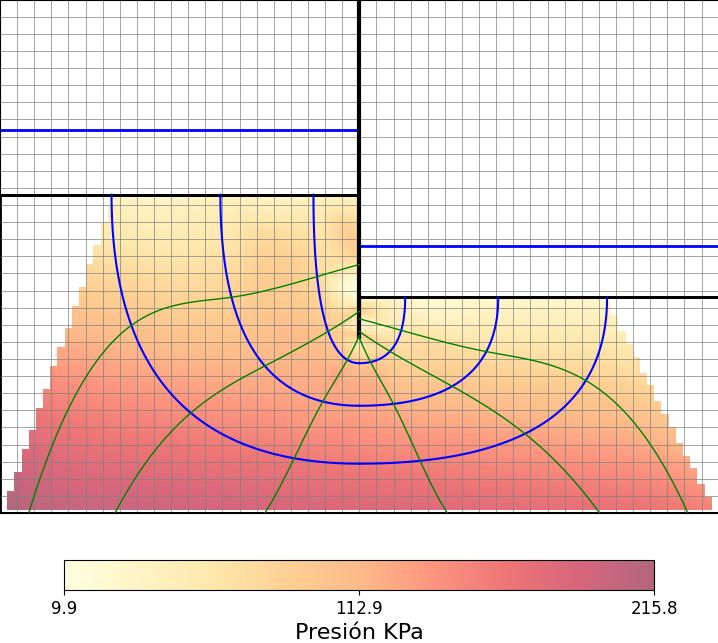
\includegraphics[width=\textwidth]{FOTOS/caso_2_mapa_calor.jpg}
      \caption{Caso 2 Presiones de Poros}
  \end{minipage}
  \begin{minipage}{0.32\textwidth}
      \centering
      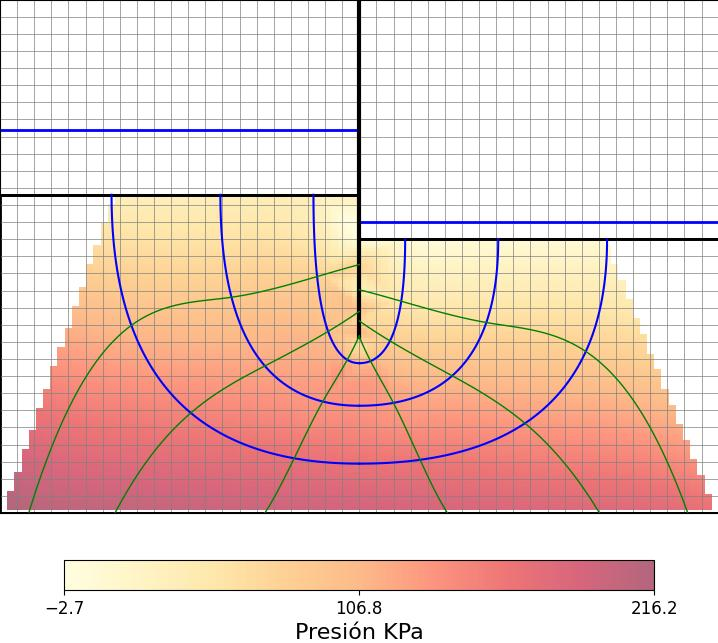
\includegraphics[width=\textwidth]{FOTOS/caso_3_mapa_calor.jpg}
      \caption{Caso 3 Presiones de Poros}
  \end{minipage}
\end{figure}

\subsubsection{Presiones Netas}

\begin{figure}[H]
  \centering
  \begin{minipage}{0.32\textwidth}
      \centering
      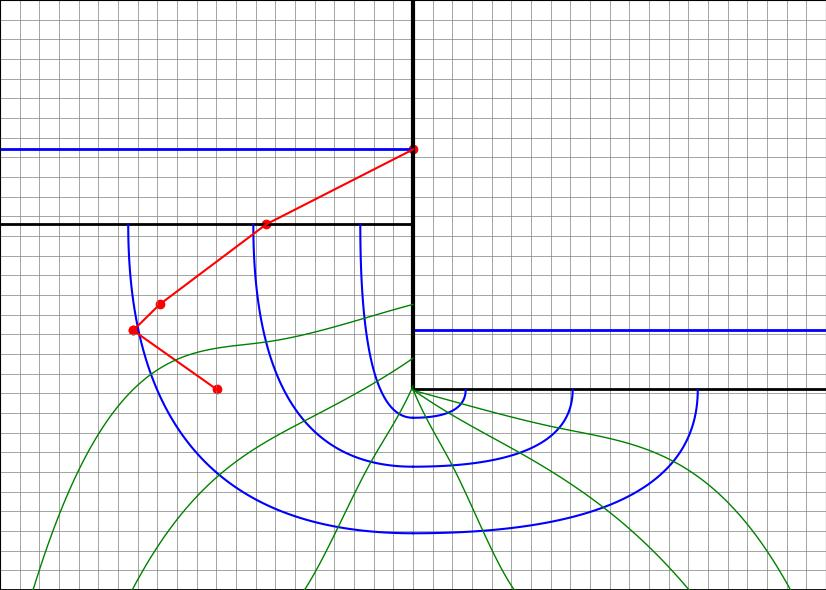
\includegraphics[width=\textwidth]{FOTOS/caso_1_presion_ataquia_neta.jpg}
      \caption{Caso 1 Presiones Ataguía Neta}
  \end{minipage}
  \begin{minipage}{0.32\textwidth}
      \centering
      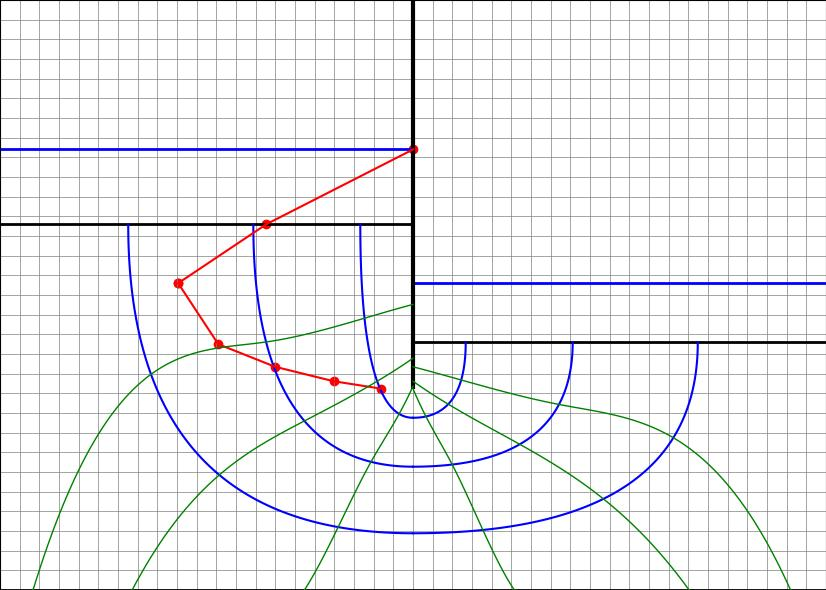
\includegraphics[width=\textwidth]{FOTOS/caso_2_presion_ataquia_neta.jpg}
      \caption{Caso 2 Presiones Ataguía Neta}
  \end{minipage}
  \begin{minipage}{0.32\textwidth}
      \centering
      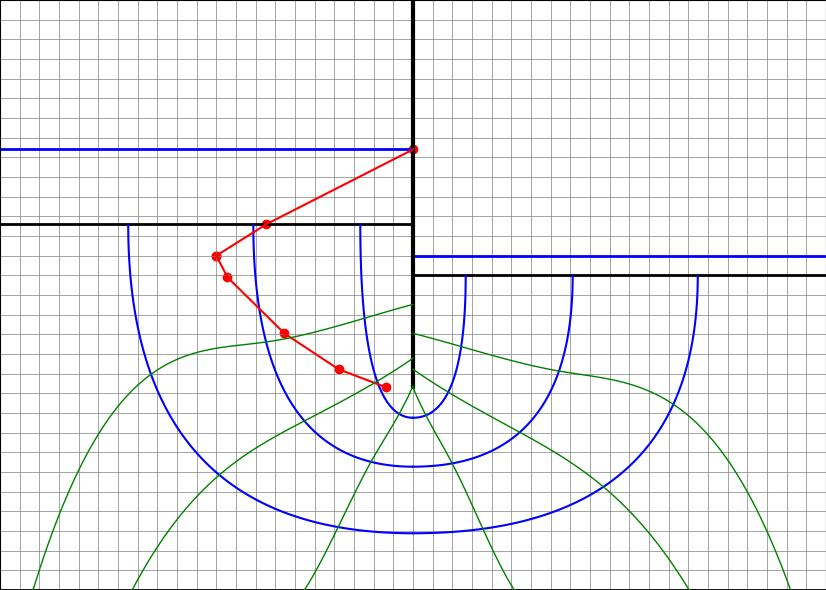
\includegraphics[width=\textwidth]{FOTOS/caso_3_presion_ataquia_neta.jpg}
      \caption{Caso 3 Presiones Ataguía Neta}
  \end{minipage}
\end{figure}

De lo cual es posible conocer el equilibrio estático de la ataguía:

\subsubsection{Centroide de la Distribución de Presiones}

La siguiente función en Python permite conocer el centroide de una función:

\begin{lstlisting}[language=Python]
  import numpy as np
  from scipy.integrate import simps

  # Calcular el área bajo la curva usando integración numérica (Simpson)
  area = simps(y, x)

  # Centroide en x
  x_bar = simps(x * y, x) / area
  
\end{lstlisting}

De lo cual se obtiene lo siguiente:

\begin{figure}[H]
  \centering
  \begin{minipage}{0.32\textwidth}
      \centering
      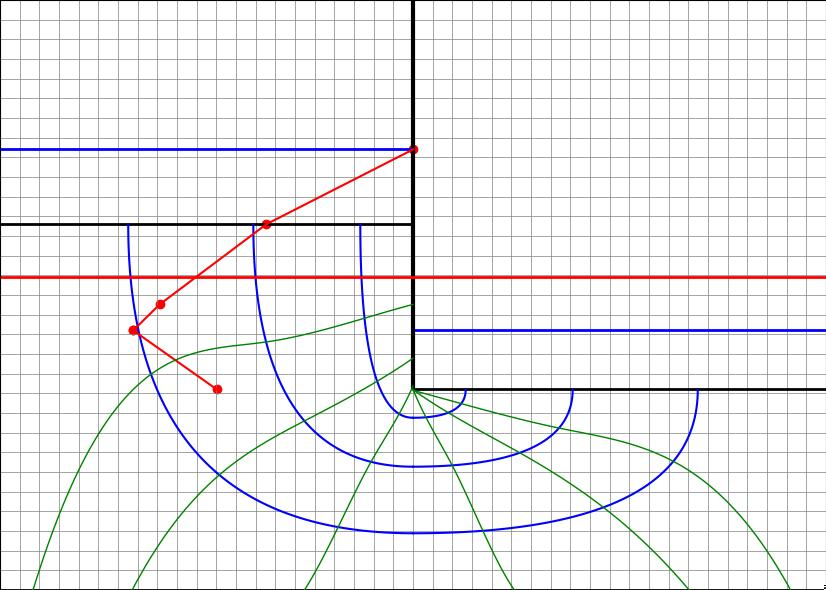
\includegraphics[width=\textwidth]{FOTOS/caso_1_centroide_y.jpg}
      \caption{Caso 1 Centroide Presiones}
  \end{minipage}
  \begin{minipage}{0.32\textwidth}
      \centering
      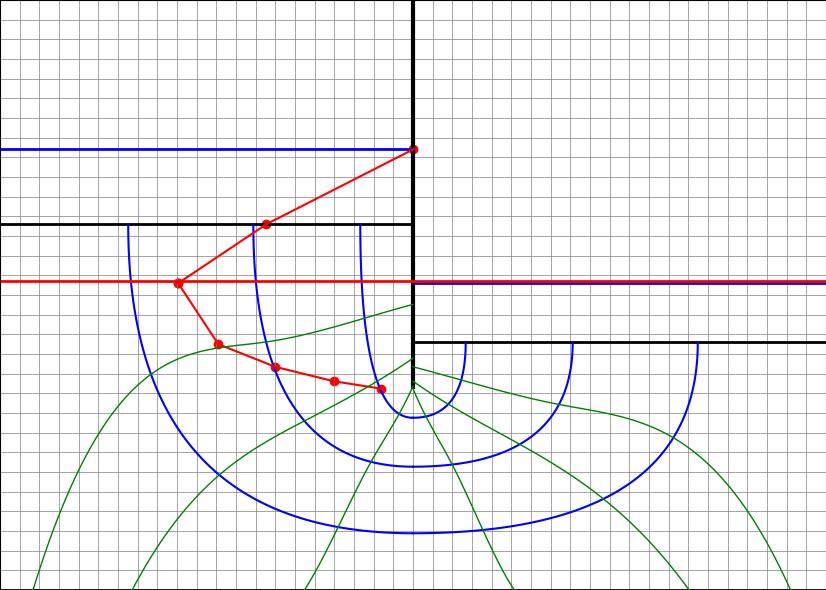
\includegraphics[width=\textwidth]{FOTOS/caso_2_centroide_y.jpg}
      \caption{Caso 2 Centroide Presiones}
  \end{minipage}
  \begin{minipage}{0.32\textwidth}
      \centering
      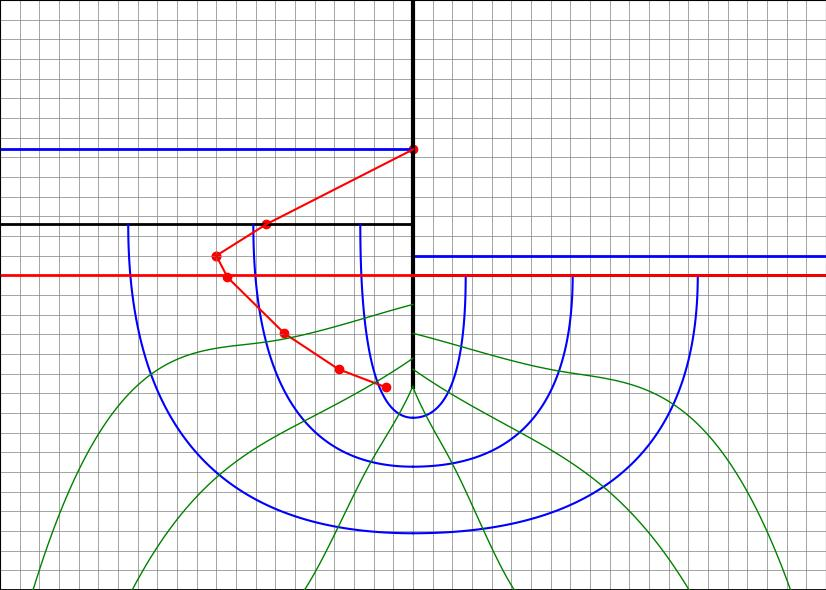
\includegraphics[width=\textwidth]{FOTOS/caso_3_centroide_y.jpg}
      \caption{Caso 3 Centroide Presiones}
  \end{minipage}
\end{figure}

Donde se puede observar que el caso 3 presenta una estabilidad en cuanto al momento neto, aun así, la estabilidad final de la ataguía dependerá de otros factores como la forma completa estructural, ya que solo estamos observando un corte transversal en este caso.

\subsection{Máximo Gradiente Hidráulico}

Se calculó el máximo gradiente hidráulico como:

\begin{lstlisting}[language=Python]
  max_g = Delta_H/((C1-C2) + 2*D)
  #es decir, DeltaH sobre el mínimo recorrido posible entre 
  #los dos puntos, donde delta_H ya fue definido anteriormente
\end{lstlisting}

De lo cual se obtuvo:

\begin{table}[H]
  \centering
  \begin{tabular}{|c|c|}
    \hline
    Caso & Máximo Gradiente Hidráulico \\
    \hline
    1 & 1.095 \\ \hline
    2 & 0.629 \\ \hline
    3 & 0.380 \\
    \hline
  \end{tabular}
  \caption{Máximo Gradiente Hidráulico}
\end{table}

\subsection{Falla por Licuefacción}

Es el proceso de cambio físico en el que un material o sustancia en estado sólido pasa a comportarse como un líquido \textbf{\cite{WebReference2024}}.
\\ \\
Los resultados obtenidos son los siguientes:

\begin{table}[H]
  \centering
  \begin{tabular}{|c|c|c|}
    \hline
    Caso & ic & Licuefacción\\
    \hline
    1 & 1.141 & No ocurre \\ \hline
    2 & 1.141 & No ocurre \\ \hline
    3 & 1.141 & No ocurre \\
    \hline
  \end{tabular}
  \caption{Falla por Licuefacción}
\end{table}

\subsection{Factor de Seguridad}

Para determinar el factor de seguridad, simplemente se calcula la relación entre ic y el máximo gradiente hidráulico:

\begin{table}[H]
  \centering
  \begin{tabular}{|c|c|}
    \hline
    Caso & FS \\
    \hline
    1 & 1.041 \\ \hline
    2 & 1.811 \\ \hline
    3 & 2.995 \\
    \hline
  \end{tabular}
  \caption{Factor de Seguridad}
\end{table}

\subsection{Análisis de Resultados}

Aunque no ocurre licuefacción en ningún caso, eso no implica una seguridad como tal en la ataguía, ya que estáticamente debe ser estable. En base a esto, se determina que el caso 3 es el más seguro, ya que la ataguía se encuentra en un equilibrio estático luego de realizar un análisis de presiones y momentos.
\\ \\
Adicionalmente, se realizó un mapa de calor sobre las presiones de poro, donde comparando con la teoría se observa una relación y afirmación de los resultados obtenidos, por lo tanto, se puede concluir que los cálculos fueron correctamente realizados.
\\ \\
En base al código realizado, este se escribió de manera personal, donde se utilizó la herramienta ChatGPT para la redacción a gran escala del código, además de la implementación de algunas librerías desconocidas. Luego, la calibración y obtención de resultados se realizó de manera manual.
\\ \\
En base a la licuefacción, se observa que el caso 1 es el más inestable, donde si se reduce un poco más el máximo gradiente hidráulico, fácilmente se alcanza el ic.
\\ \\
Finalmente, se determinaron los distintos datos solicitados como las presiones de poros en distintos puntos, o el caudal necesario de bombeo. Esta última variable dependerá del tipo de suelo, además de la instalación y gradiente hidráulico generado por la ataguía.
\\ \\
\textbf{Nota:} Los resultados dependerán mucho de la cantidad de canales de flujo y líneas equipotenciales, donde aun así se debería mantener una relación por equipotencialidad. Aun así, puede que exista una variación de los resultados en base a los inputs ingresados.

\section{Conclusión}

En conclusión, ya que todos los objetivos propuestos y solicitados fueron logrados, se puede considerar que la experiencia fue realizada de manera satisfactoria.
\\ \\
En primer lugar, personalmente me di el desafío de hacer todo el análisis mediante Python, lo cual agrega una complejidad extra al desarrollo de la entrega, donde no solo se logró tal propuesta, sino que se logró extraer información adicional a la solicitada, permitiendo así generar un análisis más completo y detallado.
\\ \\
Respecto a los cálculos realizados, se determinaron los distintos parámetros, con sus gráficas respectivas, donde el porcentaje de error aún es desconocido, ya que es necesario comparar el modelo computacional con una simulación a escala, lo cual se realizará en una futura entrega.
\\ \\
Finalmente, se logró generar un análisis crítico de los resultados y cálculos obtenidos, donde se concluye que el caso más estable es el número 3, y el más inestable el número 1.


\part{Entrega 1}

\begin{center}
    \href{https://github.com/LukasWolff2002/PROYECTO_1_MCOC_ENTREGA_1}{Ver repositorio GitHub.}
\end{center}

\setcounter{section}{0}

\section{Introducción}

\section{Marco Teórico}



\section{Desarollo}

\subsection{Caso 1}

\begin{figure}[H]
    \centering
    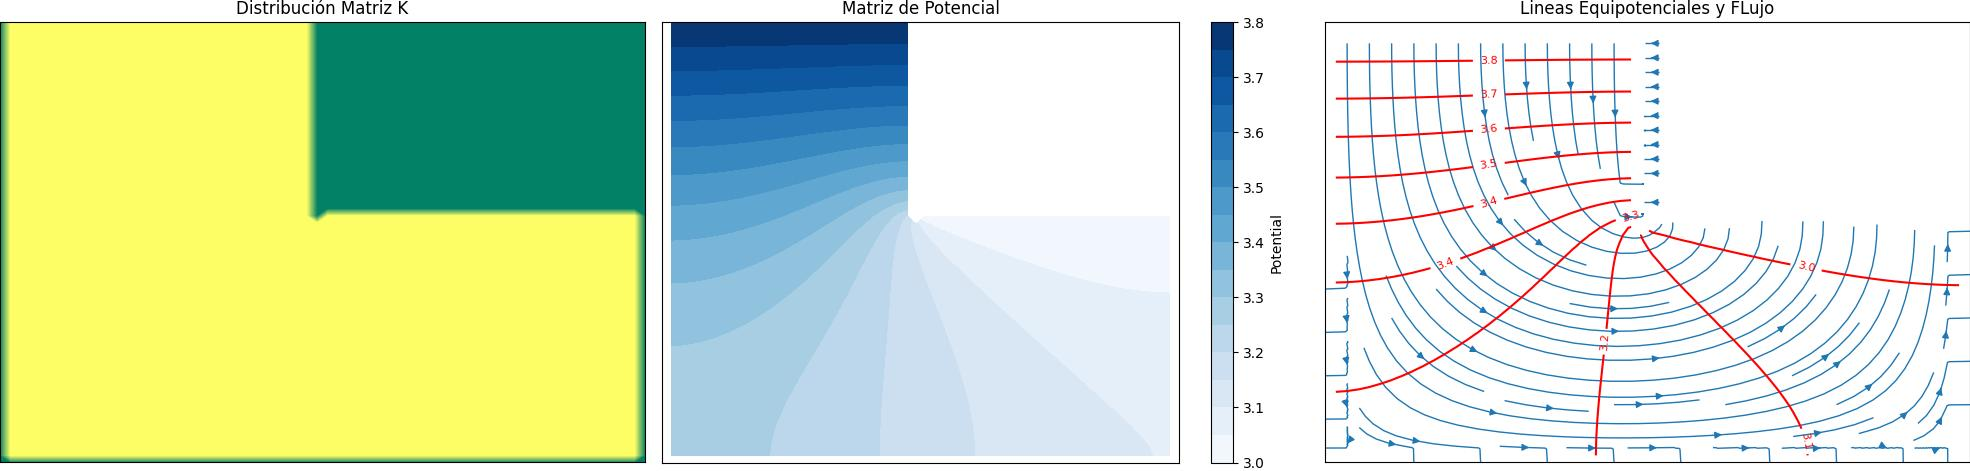
\includegraphics[width=1\textwidth]{GRAFICOS/laplace_caso_1.jpg}
    \caption{Gráfico de la función $f(x) = x^2$}
    \label{fig:caso_1}
\end{figure}

Se alcanzo la convergencia en la \textbf{iteracion 10588}
\\ \\
La velocidad de salida obtenida fue de \textbf{2.44e-05} m/s

\subsection{Caso 2}

\begin{figure}[H]
    \centering
    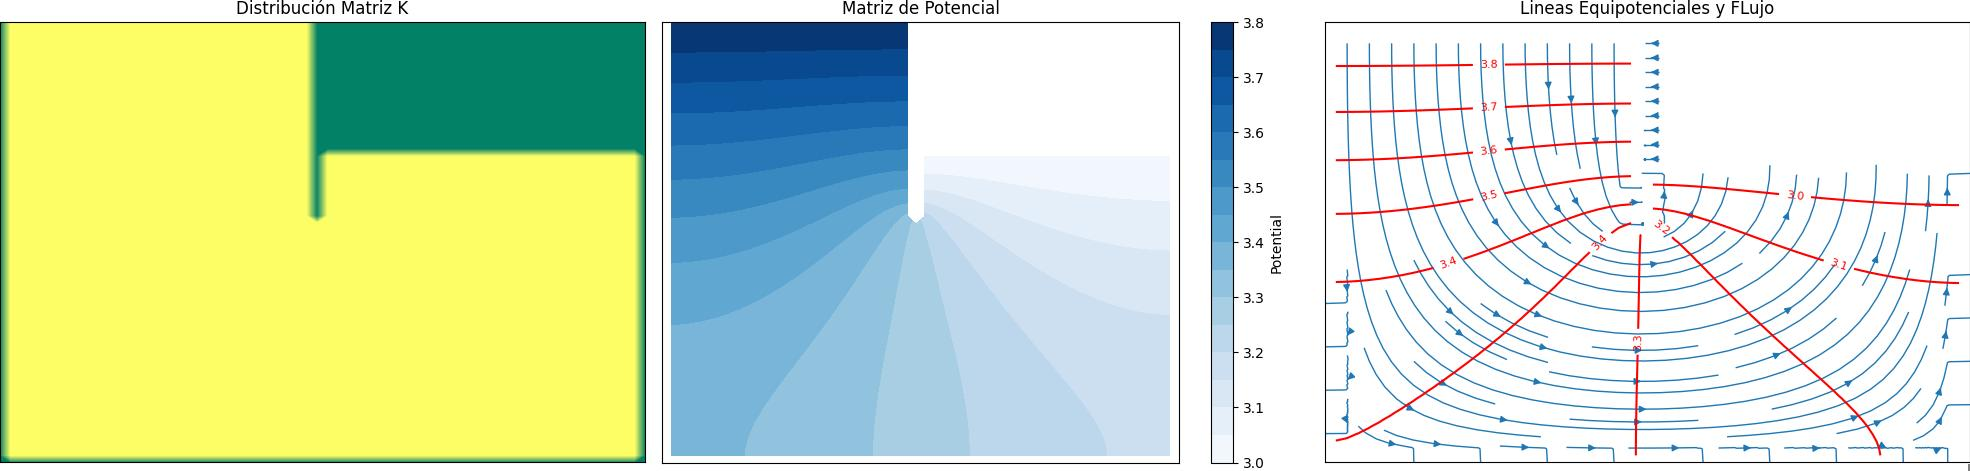
\includegraphics[width=1\textwidth]{GRAFICOS/laplace_caso_2.jpg}
    \caption{Gráfico de la función $f(x) = x^2$}
    \label{fig:caso_2}
\end{figure}

Se alcanzo la convergencia en la \textbf{iteracion 15651}
\\ \\
La velocidad de salida obtenida fue de \textbf{2.71e-05} m/s

\subsection{Caso 3}

\begin{figure}[H]
    \centering
    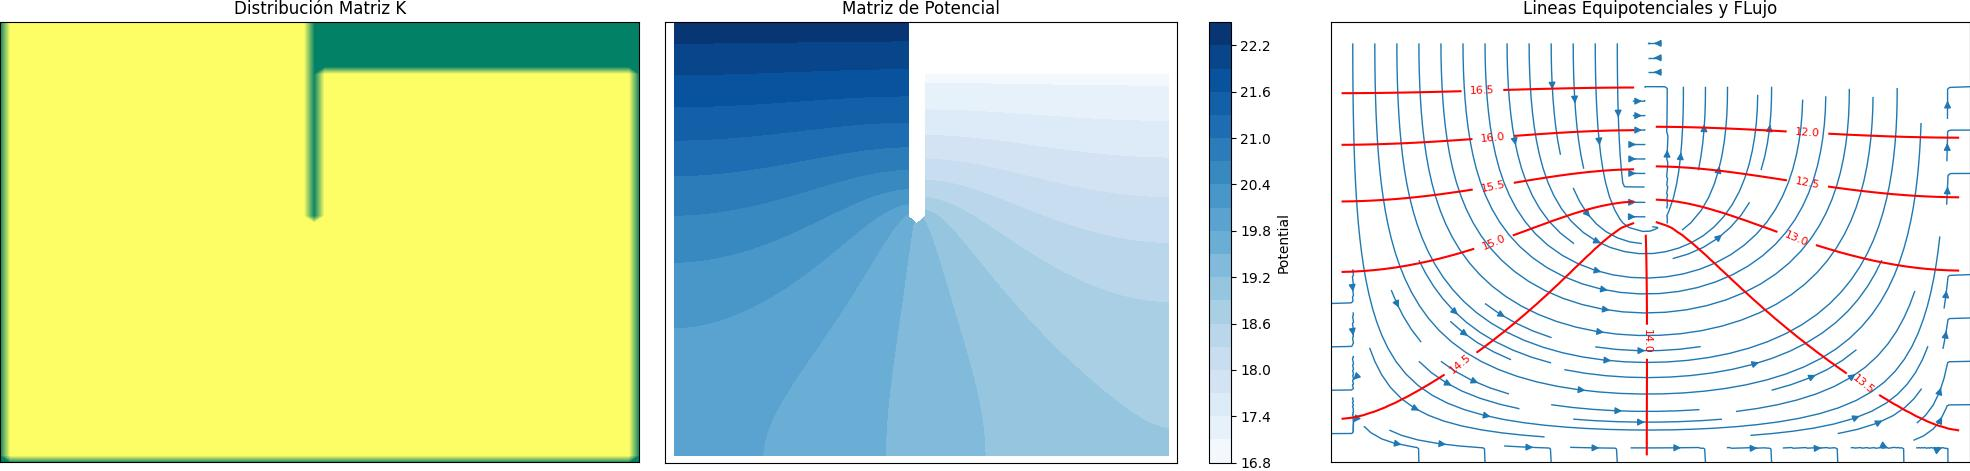
\includegraphics[width=1\textwidth]{GRAFICOS/laplace_caso_3.jpg}
    \caption{Gráfico de la función $f(x) = x^2$}
    \label{fig:caso_3}
\end{figure}

Se alcanzo la convergencia en la \textbf{iteracion 24670}
\\ \\
La velocidad de salida obtenida fue de \textbf{8.01e-05} m/s

\subsection{Caso Ejemplo Libro}

\begin{figure}[H]
    \centering
    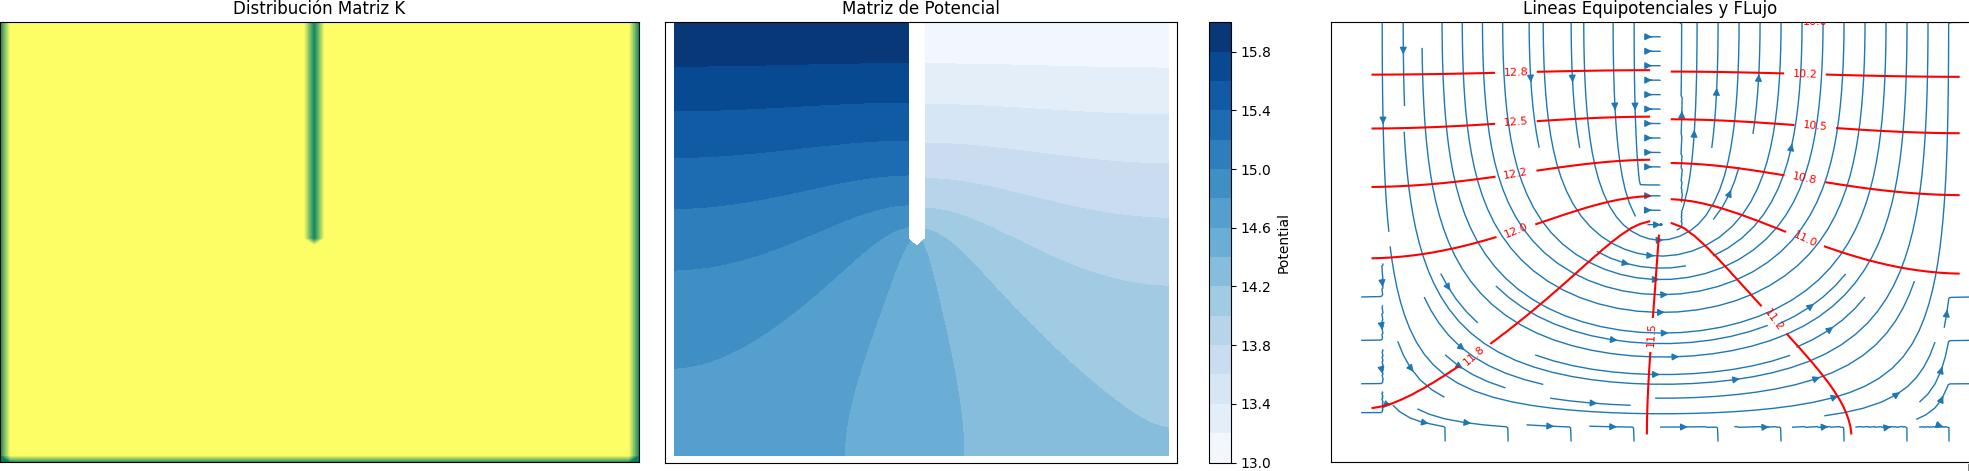
\includegraphics[width=1\textwidth]{GRAFICOS/laplace_caso_ejemplo.jpg}
    \caption{Gráfico de la función $f(x) = x^2$}
    \label{fig:caso_ejemplo}
\end{figure}

Se alcanzo la convergencia en la \textbf{iteracion 28172}
\\ \\
La velocidad de salida obtenida fue de \textbf{3.25e-06} m/s, de esta manera se corrobora que el codigo esta correctamente calibrado, ya que el resultado expuesto por el libro es de \textbf{3.2e-06} m/s.
\\ \\
Ademas, se realiza un caso doble, para ver como afecta la condicion de impermeabilidad de la barrera derecha en el flujo:

\begin{figure}[H]
    \centering
    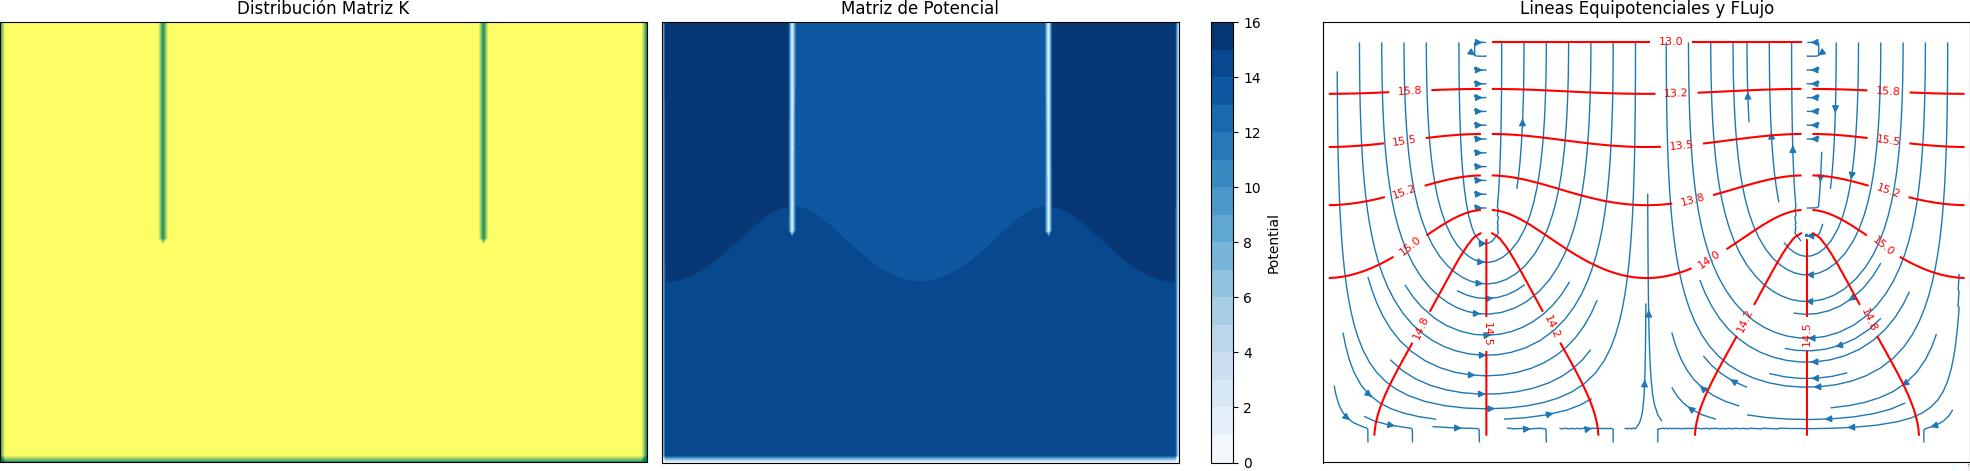
\includegraphics[width=1\textwidth]{GRAFICOS/laplace_caso_ejemplo_doble.jpg}
    \caption{Gráfico de la función $f(x) = x^2$}
    \label{fig:caso_ejemplo}
\end{figure}

Se alcanzo la convergencia en la \textbf{iteracion 16708}
\\ \\
La velocidad de salida obtenida fue de \textbf{2.63e-06} m/s.

\newpage
\bibliography{referencias}  % Nombre del archivo .bib

\end{document}
